\documentclass[onesided]{article}\usepackage[]{graphicx}\usepackage[]{color}
% maxwidth is the original width if it is less than linewidth
% otherwise use linewidth (to make sure the graphics do not exceed the margin)
\makeatletter
\def\maxwidth{ %
  \ifdim\Gin@nat@width>\linewidth
    \linewidth
  \else
    \Gin@nat@width
  \fi
}
\makeatother

\definecolor{fgcolor}{rgb}{0.345, 0.345, 0.345}
\newcommand{\hlnum}[1]{\textcolor[rgb]{0.686,0.059,0.569}{#1}}%
\newcommand{\hlstr}[1]{\textcolor[rgb]{0.192,0.494,0.8}{#1}}%
\newcommand{\hlcom}[1]{\textcolor[rgb]{0.678,0.584,0.686}{\textit{#1}}}%
\newcommand{\hlopt}[1]{\textcolor[rgb]{0,0,0}{#1}}%
\newcommand{\hlstd}[1]{\textcolor[rgb]{0.345,0.345,0.345}{#1}}%
\newcommand{\hlkwa}[1]{\textcolor[rgb]{0.161,0.373,0.58}{\textbf{#1}}}%
\newcommand{\hlkwb}[1]{\textcolor[rgb]{0.69,0.353,0.396}{#1}}%
\newcommand{\hlkwc}[1]{\textcolor[rgb]{0.333,0.667,0.333}{#1}}%
\newcommand{\hlkwd}[1]{\textcolor[rgb]{0.737,0.353,0.396}{\textbf{#1}}}%
\let\hlipl\hlkwb

\usepackage{framed}
\makeatletter
\newenvironment{kframe}{%
 \def\at@end@of@kframe{}%
 \ifinner\ifhmode%
  \def\at@end@of@kframe{\end{minipage}}%
  \begin{minipage}{\columnwidth}%
 \fi\fi%
 \def\FrameCommand##1{\hskip\@totalleftmargin \hskip-\fboxsep
 \colorbox{shadecolor}{##1}\hskip-\fboxsep
     % There is no \\@totalrightmargin, so:
     \hskip-\linewidth \hskip-\@totalleftmargin \hskip\columnwidth}%
 \MakeFramed {\advance\hsize-\width
   \@totalleftmargin\z@ \linewidth\hsize
   \@setminipage}}%
 {\par\unskip\endMakeFramed%
 \at@end@of@kframe}
\makeatother

\definecolor{shadecolor}{rgb}{.97, .97, .97}
\definecolor{messagecolor}{rgb}{0, 0, 0}
\definecolor{warningcolor}{rgb}{1, 0, 1}
\definecolor{errorcolor}{rgb}{1, 0, 0}
\newenvironment{knitrout}{}{} % an empty environment to be redefined in TeX

\usepackage{alltt}
\usepackage[T1]{fontenc}
\linespread{1.5} % Line spacing - Palatino needs more space between lines
\usepackage{microtype} % Slightly tweak font spacing for aesthetics

\usepackage[hmarginratio=1:1,columnsep=20pt]{geometry} % Document margins
%\usepackage{multicol} % Used for the two-column layout of the document
\usepackage[hang, small,labelfont=bf,up,textfont=it,up]{caption} % Custom captions under/above floats in tables or figures
\usepackage{booktabs} % Horizontal rules in tables
\usepackage{float} % Required for tables and figures in the multi-column environment - they need to be placed in specific locations with the [H] (e.g. \begin{table}[H])

\usepackage{lettrine} % The lettrine is the first enlarged letter at the beginning of the text
\usepackage{paralist} % Used for the compactitem environment which makes bullet points with less space between them

% to ignore texts: good for thank messages and paper submissions.
      % \fbox{\phantom{This text will be invisible too, but a box will be printed arround it.}}

\usepackage{abstract} % Allows abstract customization
\renewcommand{\abstractnamefont}{\normalfont\bfseries} % Set the "Abstract" text to bold
%\renewcommand{\abstracttextfont}{\normalfont\small\itshape} % Set the abstract itself to small italic text

\usepackage[]{titlesec} % Allows customization of titles
\renewcommand\thesection{\Roman{section}} % Roman numerals for the sections
\renewcommand\thesubsection{\Roman{subsection}} % Roman numerals for subsections
\titleformat{\section}[block]{\large\scshape\centering}{\thesection.}{1em}{} % Change the look of the section titles
\titleformat{\subsection}[block]{\large}{\thesubsection.}{1em}{} % Change the look of the section titles

\usepackage{fancybox, fancyvrb, calc}
\usepackage[svgnames]{xcolor}
\usepackage{epigraph}
\usepackage{longtable}
\usepackage{pdflscape}
\usepackage{graphics}
\usepackage{pbox} % \pbox{20cm}{This is the first \\ cell}
\usepackage{amsfonts}
\usepackage{amsmath}
\usepackage{amssymb}
\usepackage{rotating}
\usepackage{paracol}
\usepackage{textcomp}
\usepackage[export]{adjustbox}
\usepackage{afterpage}
\usepackage{filecontents}
\usepackage{color}
\usepackage{latexsym}
\usepackage{lscape}       %\begin{landscape} and \end{landscape}
\usepackage{wasysym}
\usepackage{dashrule}

\usepackage{framed}
\usepackage{tree-dvips}
\usepackage{pgffor}
\usepackage[]{authblk}
\usepackage{setspace}
\usepackage{array}
\usepackage[latin1]{inputenc}
\usepackage{hyperref}     %desactivar para link rojos
\usepackage{graphicx}
\usepackage{dcolumn} % for R tables
\usepackage{multirow} % For multirow in tables
\usepackage{pifont}
\usepackage{listings}




% hypothesis / theorem package begin
\usepackage{amsthm}
\usepackage{thmtools}
\declaretheoremstyle[
spaceabove=6pt, spacebelow=6pt,
headfont=\normalfont\bfseries,
notefont=\mdseries, notebraces={(}{)},
bodyfont=\normalfont,
postheadspace=0.6em,
headpunct=:
]{mystyle}
\declaretheorem[style=mystyle, name=Hypothesis, preheadhook={\renewcommand{\thehyp}{H\textsubscript{\arabic{hyp}}}}]{hyp}

\usepackage{cleveref}
\crefname{hyp}{hypothesis}{hypotheses}
\Crefname{hyp}{Hypothesis}{Hypotheses}
% hypothesis / theorem package end


%----------------------------------------------------------------------------------------
% Other ADDS-ON
%----------------------------------------------------------------------------------------

% independence symbol \independent
\newcommand\independent{\protect\mathpalette{\protect\independenT}{\perp}}
\def\independenT#1#2{\mathrel{\rlap{$#1#2$}\mkern2mu{#1#2}}}







\hypersetup{
    bookmarks=true,         % show bookmarks bar?
    unicode=false,          % non-Latin characters in Acrobat's bookmarks
    pdftoolbar=true,        % show Acrobat's toolbar?
    pdfmenubar=true,        % show Acrobat's menu?
    pdffitwindow=true,     % window fit to page when opened
    pdfstartview={FitH},    % fits the width of the page to the window
    pdftitle={My title},    % title
    pdfauthor={Author},     % author
    pdfsubject={Subject},   % subject of the document
    pdfcreator={Creator},   % creator of the document
    pdfproducer={Producer}, % producer of the document
    pdfkeywords={keyword1} {key2} {key3}, % list of keywords
    pdfnewwindow=true,      % links in new window
    colorlinks=true,       % false: boxed links; true: colored links
    linkcolor=ForestGreen,          % color of internal links (change box color with linkbordercolor)
    citecolor=ForestGreen,        % color of links to bibliography
    filecolor=ForestGreen,      % color of file links
    urlcolor=ForestGreen           % color of external links
}

%\usepackage[nodayofweek,level]{datetime} % to have date within text

\newcommand{\LETT}[3][]{\lettrine[lines=4,loversize=.2,#1]{\smash{#2}}{#3}} % letrine customization



% comments on margin
  % Select what to do with todonotes: 
  % \usepackage[disable]{todonotes} % notes not showed
  \usepackage[draft]{todonotes}   % notes showed
  % usage: \todo{This is a note at margin}

\usepackage{cooltooltips}

%%% bib begin
\usepackage[american]{babel}
\usepackage{csquotes}
\usepackage[backend=biber,style=authoryear,dashed=false,doi=false,isbn=false,url=false,arxiv=false]{biblatex}
%\DeclareLanguageMapping{american}{american-apa}
\addbibresource{/Users/hectorbahamonde/Bibliografia_PoliSci/library.bib} 
\addbibresource{/Users/hectorbahamonde/Bibliografia_PoliSci/Bahamonde_BibTex2013.bib} 

% USAGES
%% use \textcite to cite normal
%% \parencite to cite in parentheses
%% \footcite to cite in footnote
%% the default can be modified in autocite=FOO, footnote, for ex. 
%%% bib end

\usepackage{fancyhdr} % Headers and footers
\pagestyle{fancy} % All pages have headers and footers
\fancyhead{} % Blank out the default header
\fancyfoot{} % Blank out the default footer
\fancyhead[C]{Probabilidad e Incertidumbre} % Custom header text
\fancyfoot[RO,LE]{\thepage} % Custom footer text
\IfFileExists{upquote.sty}{\usepackage{upquote}}{}
\begin{document}
% DOCUMENT ID
%----------------------------------------------------------------------------------------
%	CONTENT
%----------------------------------------------------------------------------------------

%\graphicspath{
%{/Users/hectorbahamonde/RU/Term5/Experiments_Redlawsk/Experiment/Data/}
%}



%%%%%%%%%%%%%%%%%%%%%%%%%%%%%%%%%%%%%%%%%%%%%%
% begin knitr stuff


%%%%%%%%%%%%%%%%%%%%%%%%%%%%%%%%%%%%%%%%%%%%%%





\hspace{-5mm}{\bf Profesor}: H\'ector Bahamonde, PhD.\\
\texttt{e:}\href{mailto:hector.bahamonde@uoh.cl}{\texttt{hector.bahamonde@uoh.cl}}\\
\texttt{w:}\href{http://www.hectorbahamonde.com}{\texttt{www.hectorbahamonde.com}}\\
{\bf Curso}: MLE.\\
\hspace{-5mm}{\bf TA}: Gonzalo Barr\'ia.


\section{Probabilidad e Incertidumbre}

Existen tres axiomas del modelo de probabilidad. Los axiomas no son ni verdaderos ni falsos, ``simplemente son''. Desde estos tres axiomas, se puede derivar todo el resto de la teor\'ia de probabilidad.

\begin{enumerate}
  \item Para cualquier evento $z$, $Pr(z) \geq 0$. % For any event Zki, Pr(zki) 2:: O
  \item  $Pr(\mathcal{C}) \;=\; 1$.  % Sample space
  \item Si todos los eventos $K$ son mutuamente independientes, $Pr(z_{1} \;\cup\;  z_{2} \;\cup\; z_{3} \;\cup\; \;\ldots\; z_{K}) \;=\; Pr(z_{1}) \;+\; Pr(z_{2})  \;+\; Pr(z_{3}) \;\ldots\; Pr(z_{K})$
\end{enumerate}

\section{Distribuciones de Probabilidades Univariadas}

En MLE, es fundamental pensar en el ``underlying process generating [the data]''. \emph{Qu\'e tipo de proceso est\'a generando los datos?} Por ej., que una moneda de cara (1) o sello (0), se puede mencionar con la siguiente notaci\'on:

\begin{equation} 
\begin{split}
Pr(Y_{i} \;=\; 1) & = \pi \\
Pr(Y_{i} \;=\; 0) & = 1\;-\;\pi 
\end{split}
\end{equation}

donde $\pi$ es el par\'ametro (lo que estimamos) de la distribuci\'on (el mont\'on de 1's y 0's). Nuestro parametro en modelos lineales OLS era $\beta$. Ahora en MLE es $\pi$. El valor esperado de este evento $z$ (cuando la moneda no est\'a cargada) es $0.5$, o m\'as formalmente, $\pi\;=\;0.5$. {\color{red}Por qu\'e?}

\paragraph{}Este proceso se llama ``Bernoulli''.

\subsection{Bernoulli}

Bernoulli es un tipo especial de distribuci\'on ``binomial'' (de dos resultados). En general, siempre son 1's o 0's (pero puede ser cualquier otro numero---al final del d\'ia, es una distribuci\'on ``categorica''). {\color{red}Ejemplos?} 

Lo importante es que:

\begin{enumerate}
\item La probabilidad de cada evento es mayor a 0. 
\item Los posibles resultados son {\color{red}exhaustivos (?)}. O lo que es lo mismo, $Pr(Y\;=\;1 | Y\;=\;0)\;=\;0$.
\end{enumerate}



\begin{knitrout}
\definecolor{shadecolor}{rgb}{0.969, 0.969, 0.969}\color{fgcolor}\begin{kframe}
\begin{alltt}
\hlcom{# Normal }
\hlstd{binomial.ok} \hlkwb{=} \hlkwd{rbinom}\hlstd{(}
        \hlnum{100}\hlstd{,} \hlcom{# N}
        \hlnum{1}\hlstd{,} \hlcom{# pruebas (se tira la moneda una vez)}
        \hlnum{0.5} \hlcom{# probabilidad de obtener 1. }
        \hlstd{)}
\hlkwd{hist}\hlstd{(binomial.ok,} \hlkwc{main} \hlstd{=} \hlstr{""}\hlstd{)}
\end{alltt}
\end{kframe}

{\centering 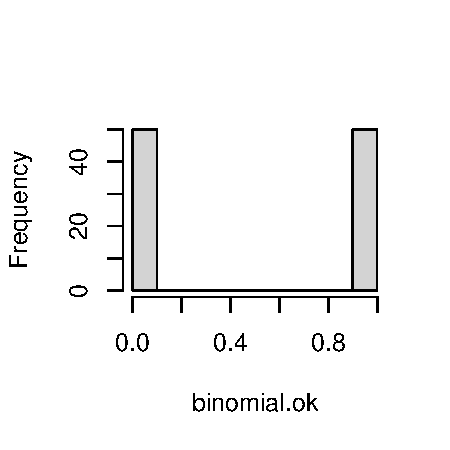
\includegraphics[width=\maxwidth]{figure/bernoulli-1} 

}


\begin{kframe}\begin{alltt}
\hlcom{# Cargada }
\hlstd{binomial.cargada} \hlkwb{=} \hlkwd{rbinom}\hlstd{(}
        \hlnum{100}\hlstd{,} \hlcom{# N}
        \hlnum{1}\hlstd{,} \hlcom{# pruebas (se tira la moneda una vez)}
        \hlnum{0.1} \hlcom{# probabilidad de obtener 1. }
\hlstd{)}
\hlkwd{hist}\hlstd{(binomial.cargada,} \hlkwc{main} \hlstd{=} \hlstr{""}\hlstd{)}
\end{alltt}
\end{kframe}

{\centering 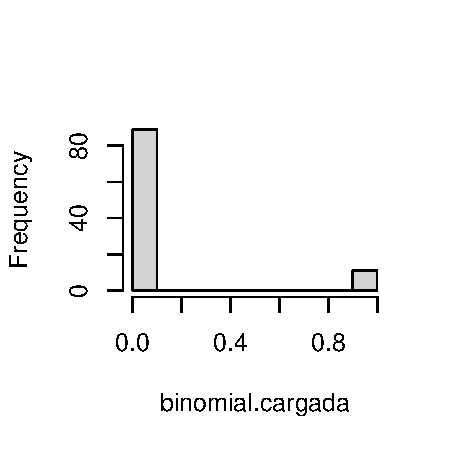
\includegraphics[width=\maxwidth]{figure/bernoulli-2} 

}



\end{knitrout}



\clearpage
\newpage
\pagenumbering{arabic}
\setcounter{page}{1}






\end{document}


